\documentclass[10pt,a4paper]{article}
\usepackage{ctex}
\usepackage{fancyhdr}
\usepackage{booktabs}
\usepackage{graphicx}
\usepackage{amsmath}
\usepackage{float}
\usepackage{xcolor}
\usepackage{listings}
\usepackage{multirow}
\usepackage{diagbox}
\usepackage[table]{xcolor}
\usepackage[colorlinks,linkcolor=blue]{hyperref} % 用于插入超链接

% 文章页面margin设置
\usepackage[a4paper]{geometry}
\geometry{top=1in}
\geometry{bottom=1in}
\geometry{left=0.75in}
\geometry{right=0.75in}   % 设置上下左右页边距
\geometry{marginparwidth=1.75cm}    % 设置边注距离(注释、标记等)

% 设置页眉
\pagestyle{fancy}
\fancyhf{}
\lhead{《人工智能基础》课程实验报告}
\chead{王荦璠,朱首赫}
\rhead{\thepage}
\renewcommand{\headrulewidth}{0.4pt}

% 代码设置
\lstset{
    basicstyle=\ttfamily\small,
    numbers=left,
    numberstyle=\tiny,
    keywordstyle=\color{blue},
    commentstyle=\color{green!60!black},
    stringstyle=\color{red},
    breaklines=true,
    frame=single,
    showstringspaces=false
}

\begin{document}

\begin{center}
    \LARGE{\textbf{《人工智能基础》课程实验报告}}
    
    \vspace{0.5cm}
    \large{王荦璠,朱首赫}
    
    \vspace{0.3cm}
    \today
\end{center}

\section{完成情况概述}
本组选择的课题为“个性化标题生成任务”,通过搭建github仓库进行协作开发,目前已完成了两个备选技术路线,包括PENS基线方法复现与改进、基于提示工程的大模型个性化生成方法。现有可运行的完整代码和清晰的Readme文档,及自行设计的创新评估方案。

\section{PENS基线方法复现与改进}
\subsection{环境搭建}
本地环境已配置 CUDA 11.8,以满足深度学习任务中对 GPU 加速的需求。考虑到项目涉及多种深度学习库(包括 PyTorch、Transformers、NumPy 等),为保障依赖管理的稳定性与可复现性,采用 Conda 作为环境管理工具,并依据基线项目提供的 requirements.txt 文件构建了独立的虚拟环境。。

\subsection{基线方法分析}
\subsubsection{整体架构}
项目遵循一个经典的三阶段流水线架构:数据预处理 (Preprocess) -> 用户建模 (UserEncoder) -> 个性化生成 (Generator)。开始时,原始数据存储在 ‘data/’ 目录中,首先需要‘Preprocess’ 组件将原始数据清洗、转换并结构化,输出到 ‘data2/’ 目录,这个目录下的数据是后续所有模型训练的直接数据源。然后‘UserEncoder’ 和 ‘Generator’ 组件分别进行模型训练,并将训练好的模型(即组件的产物)保存在 ‘runs/’ 目录下的相应子目录中。这个过程中,下游组件明确依赖上游组件的产物:‘UserEncoder’ 依赖 ‘data2/’ 的数据,而 ‘Generator’ 则同时依赖 ‘data2/’ 的数据和 ‘UserEncoder’ 训练出的模型。
\subsubsection{核心组件分析}
\textbf{数据预处理 (Preprocess):}在 PENS 个性化新闻标题生成项目中,数据预处理(Preprocess)组件是整个工作流的起点,其核心逻辑集中在 pensmodule/Preprocess/preprocess.ipynb 中。该组件的主要职责是将原始的、非结构化的新闻文本和用户行为日志转化为深度学习模型可接受的标准化数值格式。其内部由多个功能模块组成,虽非独立 Python 脚本,但通过 Jupyter Notebook 的代码单元顺序执行形成了完整的流水线。首先,环境配置模块导入必要的库(如 pandas、numpy、nltk、torch)并定义全局超参数(如 MAX\_CONTENT\_LEN, WORD\_FREQ\_THRESHOLD 等),为数据处理流程设定统一标准。接着,新闻解析模块(read\_news)读取原始 news.tsv 文件,执行文本清洗、分词、词频统计,并构建 word\_dict、category\_dict、news\_index 等核心词典映射。随后,这些词典和索引信息被序列化保存至磁盘,作为项目中的首个数据检查点。为满足下游模型输入格式,Preprocess 分别为用户编码器(UserEncoder)和标题生成器(Generator)生成不同的数据表示。前者生成固定长度的新闻标题、正文和类别 ID 序列并保存为 .npy 文件,后者则构建 Seq2Seq 模型所需的源-目标对,包含正文输入、标题输入与输出序列。此外,组件还通过加载预训练 GloVe 向量为项目构建词嵌入矩阵,并处理用户点击日志,生成用户点击历史和训练样本,包括正负样本配对。最终,这些用户数据也被序列化存储,成为后续模型训练的基础。整个 Preprocess 组件通过内存变量传递与文件系统持久化相结合的方式,确保数据处理的连续性、结构的清晰性和下游可复用性,是实现项目个性化生成能力的坚实数据基础。

\textbf{用户编码器(UserEncoder):}
该组件承担着“理解用户”的核心职责,其目标是将用户的历史点击行为转化为一个固定维度的用户兴趣向量(User Vector),用于指导下游的标题生成模型。该组件以 Preprocess 组件生成的结构化数据为输入,最终输出一个训练好的深度学习模型,逻辑分布于多个 Python 文件中,并由 Jupyter Notebook(pipeline\_Train\_Test.ipynb)协调执行。其工作流程首先由 data.py 负责数据加载,它将 .npy 和 .pkl 文件构造成可供 PyTorch 使用的 Dataset 和 DataLoader,其中每个训练样本包括候选新闻、用户点击历史及其标签。随后,modules.py 定义了多头注意力(MultiHeadAttention)和注意力池化(AttentionPooling)等通用网络结构,为 model.py 中的核心模型(如 NRMS)提供构建模块。model.py 则定义了新闻编码器和用户编码器的具体结构,利用词嵌入初始化、注意力机制等方法提取用户兴趣表示。辅助模块 utils.py 提供模型训练过程中的准确率评估函数,而训练的总流程则集中在 pipeline\_Train\_Test.ipynb 中,包括环境配置、数据加载、模型初始化、迭代训练、性能评估与模型保存。整个 UserEncoder 模块高度模块化,逻辑清晰,训练产物保存在 runs/userencoder/ 目录下,并作为下游 Generator 组件生成个性化标题的重要输入。这种分工明确、耦合度低的设计使得组件易于维护、调试与替换,是实现用户个性建模的关键基础。

\textbf{个性化生成器(Generator):}
该组件是整个系统的最终执行单元,其主要任务是融合来自 Preprocess 的结构化数据与 UserEncoder 提供的用户兴趣向量,生成既符合新闻内容又契合用户偏好的个性化新闻标题。该组件采用现代自然语言生成任务中经典的“预训练-微调”两阶段策略,由多个功能模块组成并通过 pipeline\_pretrain\_train\_test.ipynb 统一调度。首先,配置文件 config.json 提供了模型结构与训练超参数的全局定义;数据加载模块 data.py 负责将结构化数据转化为适用于训练的 PyTorch Dataset,其中 Seq2SeqDataset 用于通用预训练,ImpressionDataset 则加载用户点击历史与新闻向量用于个性化微调。模型的底层构件分布于 encoder.py、decoder\_pointer.py 与 modules.py 中,分别定义了编码器、带指针机制的解码器以及通用注意力层,实现了输入新闻文本的有效表示与个性化控制能力。model.py 中的 HeadlineGen 类则将上述模块整合为一个可训练的完整模型,其 forward 函数实现了对新闻文本的编码、结合用户兴趣向量解码生成标题的全过程。训练逻辑由 train.py 和 eval.py 等模块提供支持,封装了优化器、损失函数、微调逻辑、性能评估与 Beam Search 生成策略。整个训练与评估过程在 Jupyter Notebook 中有序展开:首先利用 Seq2SeqDataset 进行预训练,学习一般性标题生成能力;随后加载训练好的 UserEncoder 模型进行微调,将用户兴趣向量注入生成流程,从而实现真正的个性化生成,并将最终模型保存在 runs/ 目录。

\subsection{基线方法改进}
\textbf{解决原代码的兼容性问题:}
在适配项目代码至 PyTorch 2.0 及以上版本时,发现原有模型加载方式存在兼容性问题。具体来说,原始代码在加载训练好的模型检查点时,直接使用 torch.load(checkpoint\_path)进行模型还原。但在 PyTorch 2.0 起,torch.load() 新增了一个默认参数 weights\_only=True,即默认仅加载模型的权重部分,而不恢复模型对象本身的结构。由于原代码并未显式指定 weights\_only=False,这会导致模型加载过程中,checkpoint['model'] 返回为 None 或空字典,从而在后续尝试调用模型属性、执行推理或微调操作时触发报错。因此,为保证代码的稳定运行与模型的完整还原,需要显式地在加载检查点时传入 weights\_only=False 参数(如下图1),以确保模型结构与权重一并加载。此修复对于后续模块(如个性化生成器中的微调与推理)能否正常运行至关重要。
\begin{figure}[H]
  \centering
  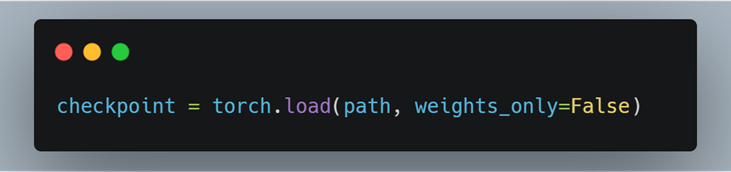
\includegraphics[width=10cm]{fig/load_new.png}
  \caption{改进后的模型加载方式}
\end{figure}

\textbf{训练方法优化:}
在复现并运行原始项目训练流程(包括 UserEncoder 训练和 Generator 的预训练/微调)时,观察到本地 GPU 使用率严重不达标,训练过程中 GPU 占用率多数时间低于 10\%,功率也接近空闲状态,仅在个别时间段出现短暂上升,但峰值也较低。这种“GPU 闲置”现象表明,训练瓶颈不在模型计算,而是数据传输过程。通过分析数据加载过程发现,原始的 DataLoader 使用的是单线程加载策略,且未启用任何内存加速机制,导致 CPU 数据准备速度无法匹配 GPU 运算速度,从而频繁阻塞 GPU 等待输入。为此,笔者对训练数据加载流程进行了两项优化:其一是设置 DataLoader 的 num\_workers 参数为系统支持的较大值(如 20),启用多线程数据加载,提升数据读取与预处理速度;其二是启用 pin\_memory=True,将数据加载到固定内存(Pinned Memory),加快 CPU 到 GPU 的数据传输速度。这一系列改进显著提升了系统吞吐能力,使 GPU 占用率长期维持在 97\%~100\%,整体训练效率提高了约一倍,尤其在数据预处理、模型预训练和个性化微调阶段的迭代速度有了显著提升。

\textbf{新增功能模块:}
为提升项目的可用性与交互性,新增了一个名为 predict\_with\_trained\_model.ipynb 的功能模块,用于实现模型的推理应用与结果输出。该模块允许用户在训练完成后,直接加载训练好的个性化标题生成模型,并对指定输入数据(可以是原始新闻正文,也可以是用户自定义文本)执行标题生成任务。生成结果会自动保存在当前目录下的 generated\_titles.txt 文件中,便于查阅与后续分析。此外,如果用户同时提供了对应的“参考标题”(即人工撰写或已有的真实标题),系统还会自动调用内置的评估函数对生成结果进行 ROUGE 指标评分,量化模型的生成质量。该模块的添加不仅提升了项目的实用性,也为实际部署、用户交互和性能评估提供了便利。

\section{标题三}

\section{实验总结}

\section{分工}
朱首赫:基线方法的复现与改进、数据集内部结构研究与分析、报告文档1-2节撰写

\end{document}